\documentclass[twoside,twocolumn]{article}

\usepackage{blindtext} % Package to generate dummy text throughout this template 
\usepackage{graphicx}
\usepackage[sc]{mathpazo} % Use the Palatino font
\usepackage[T1]{fontenc} % Use 8-bit encoding that has 256 glyphs
\linespread{1.05} % Line spacing - Palatino needs more space between lines
\usepackage{microtype} % Slightly tweak font spacing for aesthetics

\usepackage[english]{babel} % Language hyphenation and typographical rules

\usepackage[hmarginratio=1:1,top=32mm,columnsep=20pt]{geometry} % Document margins
\usepackage[hang, small,labelfont=bf,up,textfont=it,up]{caption} % Custom captions under/above floats in tables or figures
\usepackage{booktabs} % Horizontal rules in tables

\usepackage{lettrine} % The lettrine is the first enlarged letter at the beginning of the text

\usepackage{enumitem} % Customized lists
\setlist[itemize]{noitemsep} % Make itemize lists more compact

\usepackage{abstract} % Allows abstract customization
\renewcommand{\abstractnamefont}{\normalfont\bfseries} % Set the "Abstract" text to bold
\renewcommand{\abstracttextfont}{\normalfont\small\itshape} % Set the abstract itself to small italic text

\usepackage{titlesec} % Allows customization of titles
\renewcommand\thesection{\Roman{section}} % Roman numerals for the sections
\renewcommand\thesubsection{\roman{subsection}} % roman numerals for subsections
\titleformat{\section}[block]{\large\scshape\centering}{\thesection.}{1em}{} % Change the look of the section titles
\titleformat{\subsection}[block]{\large}{\thesubsection.}{1em}{} % Change the look of the section titles

\usepackage{fancyhdr} % Headers and footers
\pagestyle{fancy} % All pages have headers and footers
\fancyhead{} % Blank out the default header
\fancyfoot{} % Blank out the default footer
\fancyhead[C]{Estandar ISO SQL $\bullet$ Agosto  2019 $\bullet$ } % Custom header text
\fancyfoot[RO,LE]{\thepage} % Custom footer text

\usepackage{titling} % Customizing the title section

\usepackage{hyperref} % For hyperlinks in the PDF

%----------------------------------------------------------------------------------------
%	TITLE SECTION
%----------------------------------------------------------------------------------------

\setlength{\droptitle}{-4\baselineskip} % Move the title up

\pretitle{\begin{center}\Huge\bfseries} % Article title formatting
\posttitle{\end{center}} % Article title closing formatting
\title{Estandar ISO SQL-XXXX} % Article title
\author{Jose Luis Quispe Mamani}
\date{\today} % Leave empty to omit a date
\renewcommand{\maketitlehookd}{%
\begin{abstract}
\noindent 
In this article the new features of the ISO ISO standards will be announced, identifying and analyzing their importance, as well as the definitions and concepts of the different standards that exist, with the purpose of starting the development of this course.
\end{abstract}
\begin{abstract}
\noindent 
En el presente rticulo se dara a conocer las nuevas caracteristicas de los estandares ISO de SQL, identificando y analizando su importancia, asi como las definiciones y conceptos de los distintos estandares que hay, con el proposito de dar inicio al desarrollo de este curso.
\end{abstract}
}

%----------------------------------------------------------------------------------------

\begin{document}

% Print the title
\maketitle

%----------------------------------------------------------------------------------------
%	ARTICLE CONTENTS
%----------------------------------------------------------------------------------------

\section{Introduccion}
\lettrine[nindent=0em,lines=3]{L}as normas ISO se crearon con la finalidad de ofrecer orientacion, coordinacion, simplificacion y unificacion de criterios a las empresas y organizaciones con el objeto de reducir costes y aumentar la efectividad, asi como estandarizar las normas de productos y servicios para las organizaciones internacionales. Las normas ISO se han desarrollado y adoptado por multitud de empresas de muchos paises por una necesidad y voluntad de homogeneizar las caracteristicas y los parametros de calidad y seguridad de los productos y servicios.


%------------------------------------------------

\section{Marco Teorico}

\subsection{Que son los Estandares ISO}

Las normas ISO son un conjunto de normas orientadas a ordenar la gestión de una empresa en sus distintos ámbitos. La alta competencia internacional acentuada por los procesos globalizadores de la economía y el mercado y el poder e importancia que ha ido tomando la figura y la opinión de los consumidores, ha propiciado que dichas normas, pese a su carácter voluntario, hayan ido ganando un gran reconocimiento y aceptación internacional.Las normas ISO son establecidas por el Organismo Internacional de Estandarización (ISO), y se componen de estándares y guías relacionados con sistemas y herramientas específicas de gestión aplicables en cualquier tipo de organización.

El Organisno Internacional de Normalización (ISO) fue creado en 1947 y cuenta con 91 estados miembros, que son representados por organismos nacionales de normalización. Dicho organismo trabaja para lograr una forma común de conseguir el establecimiento del sistema de calidad, que garantice la satisfacción de las necesidades y expectativas de los consumidores.A comienzos del año 1980, la ISO designó una serie de comités técnicos para que trabajaran en el desarrollo de normas comunes que fuesen aceptadas universalmente. El resultado de este trabajo fue publicado siete años más tarde a través del compendio de normas ISO 9000, posterior a la publicación de la norma de aseguramiento de la calidad-vocabulario (ISO 8402), que fue dada a conocer en 1986.El desarrollo y diversificación de las normas ISO han sido muy importantes, desdoblándose en diferentes ramas o familias que tratan aspectos diversos como la calidad, el medio ambiente, la seguridad y riesgos laborales y la responsabilidad social. El proceso es continuo y periódicamente van apareciendo actualizaciones y nuevos ámbitos de tratamiento.

\begin{center}
	
\includegraphics[width=5cm]{./Imagenes/iso} 
\end{center}

\subsection{Que es SQL}
es un lenguaje de dominio específico utilizado en programación, diseñado para administrar, y recuperar información de sistemas de gestión de bases de datos relacionales. Una de sus principales características es el manejo del álgebra y el cálculo relacional para efectuar consultas con el fin de recuperar, de forma sencilla, información de bases de datos, así como realizar cambios en ellas.

Originalmente basado en el álgebra relacional y en el cálculo relacional, SQL consiste en un lenguaje de definición de datos, un lenguaje de manipulación de datos y un lenguaje de control de datos. El alcance de SQL incluye la inserción de datos, consultas, actualizaciones y borrado, la creación y modificación de esquemas y el control de acceso a los datos. También el SQL a veces se describe como un lenguaje declarativo, también incluye elementos procesales.

SQL fue uno de los primeros lenguajes comerciales para el modelo relacional de Edgar Frank Codd como se describió en su artículo de investigación de 1970 El modelo relacional de datos para grandes bancos de datos compartidos. A pesar de no adherirse totalmente al modelo relacional descrito por Codd, pasó a ser el lenguaje de base de datos más usado.

\begin{center}
	
\includegraphics[width=7cm]{./Imagenes/sql} 
\end{center}

%------------------------------------------------

\section{Analisis}

\subsection{SQL-86 (or SQL-87) is the ISO 9075:1987 standard of 1987}
SQL es una abreviatura de "Structured Query Language", esto es, Lenguaje de Consulta Estructurado. Con este lenguaje se
formulan operaciones relacionales, es decir, operaciones que permiten definir y manipular una base de datos relacional.
En 1986, el Instituto Nacional Norteamericano de Normalización (ANSI) publicó las primeras normas que enunciaban sintaxis y la semántica de SQL. En 1989, ANSI definió el SQL2, basado en el anterior pero con una serie de mejoras (definición de claves primarias, integridad de los datos, etc.).

\subsection{SQL-89 is the ISO/IEC 9075:1989 standard of 1989}
En 1989, ANSI definió el SQL89, basado en el anterior pero con una serie de mejoras (definición de claves primarias, integridad de los datos, etc). Una característica importante definida era la posibilidad de utilizarse a través de dos interfaces: interactivamente o dentro de programas de aplicación.

En su primera versión del SQL-89 se tienen tres partes:
\begin{itemize}	
	\item El lenguaje de definición de datos (LDD). Contiene todas las instrucciones para definir el esquema de una base de datos, como son: create, alter y drop.
	\item El lenguaje de manipulación de datos (LMD). Contiene las instrucciones de manejo de las tablas como son: select, insert, delete y update, y para control de concurrencia como: commit y rollback.
	\item El lenguaje de control de datos (LCD). Contiene aquellas instrucciones para dar y revocar permisos de acceso a los datos de la base de datos, como son: grant y revoke.
\end{itemize}

\subsection{SQL-92 is the ISO/IEC 9075:1992 standard of 1992}
SQL-92 fue desarrollado por el comité técnico NCITS H2 sobre bases de datos. Este comité desarrolla estándares para la sintaxis y semántica de los lenguajes de bases de datos. SQL-92 fue diseñado para ser un estándar para los sistemas manejadores de bases de datos relacionales (RDBMS). Esta basado en SQL-89, cuya primera versión se conoce como SQL-86. En 1992 aparece SQL2 o SQL92, la versión hoy en día más difundida ([ISO/IEC 1992] [ANSI 1992] [ISO/IEC 1994]). Con la aparición de la segunda versión del estándar (SQL2) en 1992, prácticamente todos los RDBMS, incluso los no relacionales, incluían soporte a SQL. Hoy en día, SQL se ha convertido en el lenguaje de consulta más utilizado.

\subsection{SQL:1999 is the ISO/IEC 9075:1999 standard of 1999}
 Fue la cuarta revisión del estándar SQL. Introdujo un gran número de nuevas características, muchas de las cuales requerían aclaraciones en el posterior SQL:2003. La última revisión del estándar es SQL:2011.
 
 Los documentos de la norma ISO fueron publicados entre 1999 y 2002 en varias entregas, la primera consistió en múltiples partes. A diferencia de las ediciones anteriores, el nombre del estándar usaba dos puntos en lugar de un guion para la coherencia con los nombres de otros estándars ISO. La primera versión de SQL:1999 tenía cinco partes:

\begin{itemize}	
	\item SQL/Framework ISO/IEC 9075-1:1999
	\item SQL/Foundation ISO/IEC 9075-2:1999
	\item SQL/CLI ISO/IEC 9075-3:1999
	\item SQL/PSM ISO/IEC 9075-4:1999
	\item SQL/Bindings ISO/IEC 9075-5:1999
\end{itemize}

\subsection{SQL:2003 is the ISO/IEC 9075:2003 standard of 2003}
El lenguaje estándar llamado SQL3, prometió ser un aumento de la segunda generación de SQL (comúnmente conocido como SQL92, debido al año de su publicación), SQL3 fue originalmente planeado para su uso en el año 1996, pero tardó 7 años en desarrollarse en vez de los tres o cuatro que se pensaba iba a tardar.

SQL3 está caracterizado como “SQL orientado a objetos” y es la base de algunos sistemas de manejo de bases de datos orientadas a objetos (incluyendo ORACLE, Informix Universal Server, IBM’s DB Universal Database y Cloudscape, además de otros).


\subsection{SQL:2006 is the ISO/IEC 9075:2006 standard of 2006}
Define las maneras en las cuales SQL se puede utilizar conjuntamente con XML. Define maneras de importar y guardar datos XML en una base de datos SQL, manipulándolos dentro de la base de datos y publicando el XML y los datos SQL convencionales en forma XML. Además, proporciona facilidades que permiten a las aplicaciones integrar dentro de su código SQL el uso de XQuery, lenguaje de consulta XML publicado por el W3C (World Wide Web Consortium) para acceso concurrente a datos ordinarios SQL y documentos XML.

\subsection{SQL:2008 is the ISO/IEC 9075:2008 standard of 2008}
Es la sexta revisión del estándar ISO y ANSI para el lenguaje de bases de datos SQL. Se adoptó formalmente en julio de 2008.
El estándar SQL:2008 se divide en varias partes, que abarcan el Framework, la Fundación, el SQL/CLI, SQL/PSM, SQL/MED, SQL/OLB, SQL/Schemata, SQL/JRT Using Java, y varias especificaciones relacionadas.

Propiedades añadidas
\begin{itemize}	
	\item Sentencias MERGE y DIAGNOSTIC mejoradas
	\item sentencias TRUNCATE TABLE
	\item cláusulas WHEN y expresiones CASE
	\item INSTEAD OF database trigger
	\item JOIN
	\item soporte para varias expresiones regulares XQuery
	\item mejores al nombrado de las columnas derivadas.
\end{itemize}

\subsection{SQL:2011 is the ISO/IEC 9075:2011 standard of 2011}
Datos temporales (PERIOD FOR). Mejoras en las funciones de ventana y de la cláusula FETCH.

\subsection{SQL:2016 is the ISO/IEC 9075:2016 standard of 2016}
Permite búsqueda de patrones, funciones de tabla polimórficas y compatibilidad con los ficheros JSON.

\begin{center}
	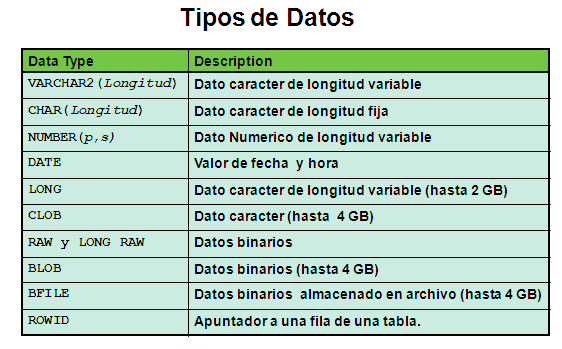
\includegraphics[width=8cm]{./Imagenes/tipo} 
\end{center}

\section{Conclusiones}
A traves del tiempo, se han mejorado las distintas herramientas que ahora conocemos para su uso correcto, y gracias a ellos, podemos aprender de una manera mas sencilla y didactica acerca de su funcionalidad y uso.

Asi tambien como los diferentes usos que se les puede dar y las diferentes informaciones que pueden proporcionar para un mejor uso de los datos.


%	REFERENCE LIST
%----------------------------------------------------------------------------------------
\begin{thebibliography}{99} % Bibliography - this is intentionally simple in this template
\bibitem[Chapple, 2015]{Chapple,Mike:2015}
\newblock Database. SQL Fundamentals.

\bibitem[Morteo, 2004]{Morteo,Francisco Agustin:2004}
Morteo,F.A y B.N.(2004).
\newblock Un enfoque practico de SQL.
\end{thebibliography}
%----------------------------------------------------------------------------------------

\end{document}
